\subsection{Choosing The Internal Architecture}
To choose a fitting architecture is a balance act and may end up limiting a project if not done correctly.
This is something we want to avoid and as such, we will be picking certain concepts from different architectural patterns, to achieve a tailor made internal architecture.

We deem that the internal architecture should have the client--server architecture as foundation.
This means that the internals of our Android app will consist of several services and clients;
where the services provides features, and the clients accesses these features and exposes them to different parts of the system or the user.

However, because we are developing an Android app, which inevitably will have some form of \ac{UI}, we want to incorporate the idea of views from the \ac{MVC} pattern.
These views will be anything that is to be presented to the user, such as playlists or playback controls.
This further separation will enable us to decouple client functionality from client presentation, and allow for testing of the clients functionality independently from the graphical presentation.

%A graphical representation of this chosen internal architecture can be seen on \cref{fig:internal_architecture}.
%Here we can see how two potential services, music and synchronization, can be interacted with from different clients.
%Furthermore it is shown how a client can have a view, i.e.~a graphical \ac{UI}.

%\begin{figure}
%    \footnotesize
%    \centering
%    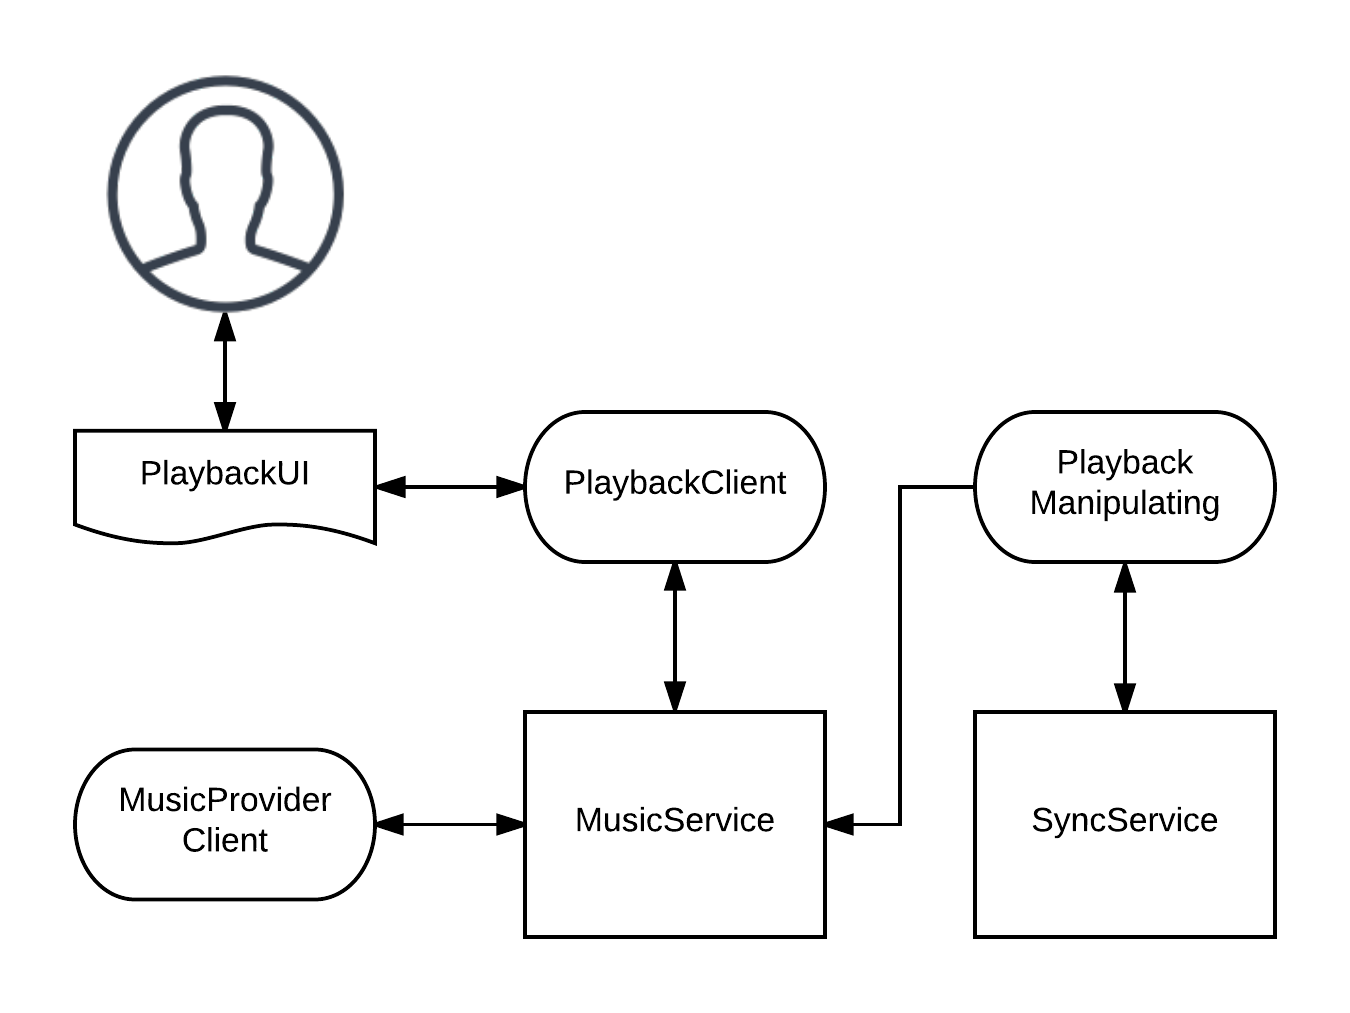
\includegraphics[width=0.8\textwidth]{img/internal_architecture.png}
%    \caption{Internal architecture, showing two potential services and how clients exist in the pattern}\label{fig:internal_architecture}
%\end{figure}
